%%%%%%%%%%%%%%%%%%%%%%%%%%%%%%%%%%%%%%%%%%%%%%%%%%%%%%%%%%%%%%%%%%%%%%%%%%%%%%%%
%   ---> This is the file you want to compile <---
%%%%%%%%%%%%%%%%%%%%%%%%%%%%%%%%%%%%%%%%%%%%%%%%%%%%%%%%%%%%%%%%%%%%%%%%%%%%%%%%

\documentclass[12pt]{report}
\usepackage{auhonors}

% this is just for lots of latin words. you probably don't need it.
\usepackage{lipsum}

% % TikZ
% \usepackage[latin1]{inputenc}
\usepackage[utf8]{inputenc}
\usepackage{tikz, tkz-euclide, pgf}
    \usetikzlibrary{calc, arrows, shapes}
    \usetkzobj{angles} % important you want to use angles

\usepackage{caption}
\captionsetup[table]{skip=10pt}

% underline emphasis in the prefatory pages
\usepackage{ulem}
% URLs...
\usepackage{url}
% enable expand math support
\usepackage{amsmath}
% enable graphic support
\usepackage{graphicx}

% table stuff
% \usepackage{array}
% \newcolumntype{$}{>{\global\let\currentrowstyle\relax}}
% \newcolumntype{^}{>{\currentrowstyle}}
% \newcommand{\rowstyle}[1]{\gdef\currentrowstyle{#1}%
%   #1\ignorespaces
% }

% for list of abbreviations
% \usepackage[intoc]{nomencl}
\usepackage{nomencl}
% used in leiu of terminal commands
\makenomenclature

% Appendices are written like regular chapters
\usepackage[toc,page]{appendix}
\appendixpageoff\appendixtocoff % keep out the useless page and toc entry

% click on links to jump in pdf - should come last of usepackages
\usepackage{hyperref}
\hypersetup{}

% May want theorems numbered by chapter
% \newtheorem{theorem}{Theorem}[chapter]

%%%%%% Define variables
\title{Latin Words Formatted for an Honors Thesis}
\author{Your Name}
\date{May 5, 2013}
\copyrightyear{2013}
\adviser{Your Advisor}
\professor{Your Advisor \\ Their Position \\ Their Department}
\professor{Constance C. Relihan \\ Associate Provost for \\ Undergraduate Studies}

\begin{document}

%%%%%%%%%%%%%%%%%%%%%%%%%%%%%%%%%%%%%%%%%%%%%%%%%%%%%%%%%%%%%%%%%%%%%%%%%%%%%%%%
%   Prefatory Pages
%%%%%%%%%%%%%%%%%%%%%%%%%%%%%%%%%%%%%%%%%%%%%%%%%%%%%%%%%%%%%%%%%%%%%%%%%%%%%%%%

\begin{romanpages}

\ApprovalPage
\TitlePage
\CopyrightPage

\begin{vita}
I was born and currently remain alive.
\end{vita}

\begin{abstract}
This paper is written using code which will be copied and pasted into other papers written by undergraduates who don't want to write their own style file.
\end{abstract}

\begin{acknowledgments}
You probably owe somebody something for getting you where you are today.
\end{acknowledgments} 

\style{ASME}
\software{\LaTeX, Ubuntu Linux 12.04.1}
\StylePage

\tableofcontents
\listoffigures
\listoftables

% nomenclature
\renewcommand{\nomname}{\sc List of Abbreviations}
\printnomenclature[0.75in]
\addcontentsline{toc}{chapter}{List of Abbreviations}

% stop using roman numerals.
\end{romanpages}

\normalem       % Make italics the default for \em


%%%%%%%%%%%%%%%%%%%%%%%%%%%%%%%%%%%%%%%%%%%%%%%%%%%%%%%%%%%%%%%%%%%%%%%%%%%%%%%%
%   Paper body
%%%%%%%%%%%%%%%%%%%%%%%%%%%%%%%%%%%%%%%%%%%%%%%%%%%%%%%%%%%%%%%%%%%%%%%%%%%%%%%%

\chapter{Latin Words}
\label{chap:latinwords}

\lipsum[1]



\section{Latin Words with a Table}
\label{sec:latinwords}

The data presented in Fig.~\ref{tab:lanechangeresults} is clearly doctored to agree with what I want it to say.


\begin{table}[htbp] \centering \caption{Cone pairs chosen in the lane change replication test}
\begin{tabular}{rc|cc} 
    GUI&    Run \#  &     Leader&    Follower \\ \hline\hline
    Earth&      1       &       1   &    3 \\
         &      2       &       3   &    4   \\ \hline
    Monolith&   3       &       2   &    3   \\
         &      4       &       5   &    5 \\ \hline   
\end{tabular} \label{tab:lanechangeresults} \end{table}

\lipsum[2]



\subsection{Latin Words \& Some Figures}
\label{sec:latinwordsfigs}

Depicted below in Figs.~\ref{fig:platypus} and \ref{fig:pangolin} are two adorable animals. 

\begin{figure}[ht] \centering
    \begin{minipage}[b]{0.45\linewidth} \centering 
        \includegraphics[width=\textwidth]{./figs/a_cute_platypus.jpg}
        \caption{Platypi swim in water often.} \label{fig:platypus}
    \end{minipage}
    \hspace{0.5cm}
    \begin{minipage}[b]{0.45\linewidth} \centering
        \includegraphics[width=\textwidth]{./figs/an_adorable_pangolin.jpg}
        \caption{The pangolin is not a fuzzy animal.} \label{fig:pangolin}
    \end{minipage}
\end{figure}

To see an animal for which an OS version was named, see Fig.~\ref{fig:quetzal} .

\lipsum[3]


%%%%%%%%%%%%%%%%%%%%%%%%%%%%%%%%%%%%%%%%%%%%%%%%%%%%%%%%%%%%%%%%%%%%%%%%%%%%%%%%
%   Appendices
%%%%%%%%%%%%%%%%%%%%%%%%%%%%%%%%%%%%%%%%%%%%%%%%%%%%%%%%%%%%%%%%%%%%%%%%%%%%%%%%

\begin{appendices}
\chapter{Miscellaneous Stuff}
\label{app:misc}



\begin{figure}[ht] \centering
    \includegraphics[width=3in]{./figs/resplendent_quetzal.jpg}
    \caption{Ubuntu 13.10 was named for the quetzal. The quantal quetzal.} \label{fig:quetzal}
\end{figure}


\begin{figure}[ht] \centering
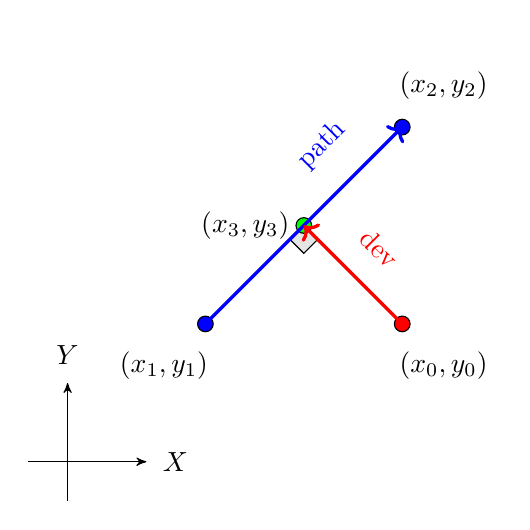
\begin{tikzpicture}[
        scale=5,
        axis/.style={thin, ->, >=stealth'},
        every node/.style={circle, color=black}   ]
    % axis
    \draw[axis] (-0.1,0) -- (0.2,0) node(xline)[right] {$X$};
    \draw[axis] (0,-0.1) -- (0,0.2) node(yline)[above] {$Y$};
    % points
    \coordinate (a) at (0.35,0.35);
    \coordinate (b) at (0.6,0.6);
    \coordinate (c) at (0.85,0.85);
    \coordinate (d) at (0.85,0.35);
    % right angle
    \tkzMarkRightAngle[fill=gray!20,size=.05](a,b,d)
    \node[draw,circle,inner sep=2pt,fill=blue] at (a) {};
    \node[draw,circle,inner sep=2pt,fill=green] at (b) {};
    \node[draw,circle,inner sep=2pt,fill=blue] at (c) {};
    \node[draw,circle,inner sep=2pt,fill=red] at (d) {};
    % point labels
    \node [below left] at (a)  {$(x_1,y_1)$};
    \node [left] at (b)  {$(x_3,y_3)$};
    \node [above right] at (c) {$(x_2,y_2)$};
    \node [below right] at (d) {$(x_0,y_0)$};
    % path arrow
    \draw[very thick,blue,->] (a) -- (c) node [pos=0.75, sloped, above, color=blue] {path};
    % dev arrow
    \draw[very thick,red,->] (d) -- (b) node [pos=0.5, sloped, above, color=red] {dev};
\end{tikzpicture}
\caption{Key path points near to the follower} \label{fig:pathpts}
\end{figure}

\end{appendices}


%%%%%%%%%%%%%%%%%%%%%%%%%%%%%%%%%%%%%%%%%%%%%%%%%%%%%%%%%%%%%%%%%%%%%%%%%%%%%%%%
%   Bib
%%%%%%%%%%%%%%%%%%%%%%%%%%%%%%%%%%%%%%%%%%%%%%%%%%%%%%%%%%%%%%%%%%%%%%%%%%%%%%%%

\bibliographystyle{asmems4}
\bibliography{thesis}

% stuff you don't cite explicitly but still want in there.
\nocite{travisdiss}
\nocite{travisshort}
\nocite{calgary}


\end{document}